\documentclass[12pt,a4paper]{article}

% Packages
\usepackage[utf8]{inputenc}
\usepackage[indonesian]{babel}
\usepackage{amsmath, amsthm, amssymb}
\usepackage{graphicx}
\usepackage{booktabs}
\usepackage{tabularx}
\usepackage{geometry}
\geometry{a4paper, margin=2.5cm}
\usepackage{hyperref}
\usepackage{xcolor}
\usepackage{titlesec}
\usepackage{float}

% Pengaturan judul
\title{
    \vspace{-2cm}
    
\includegraphics[width=4cm]{logo.png} \\[1cm]
    \textbf{Laporan Tugas Kelompok}\\
    \large Jaringan Saraf Tiruan - Logika AND \& OR dengan Perceptron
}

\author{
    \textbf{Mata Kuliah:} Kecerdasan Komputasional \\
    \textbf{Dosen Pengampu:} Dr. ARIK KURNIAWATI S.Kom., M.T \\[1cm]
    \textbf{Disusun Oleh Kelompok 6:} \\
    1. Rizki Pratama Sunarko - 240411100181 \\
    2. Ainur Suharyanto - 240411100154 \\
    3. Wahyu Ari Ananda Fitrotul Huda - 240411100148 
}
\date{\today}

\begin{document}

\maketitle
\thispagestyle{empty}

\hrule
\vspace{0.5cm}

Pada laporan tugas ini, kami menyajikan hasil penyelesaian untuk pemodelan logika AND dan OR menggunakan algoritma Jaringan Saraf Tiruan Perceptron dengan menerapkan fungsi aktivasi \textit{Step Function}.

\section{Aturan dan Parameter Pembelajaran}
Sebelum melakukan simulasi dan pelatihan model, kami menetapkan beberapa aturan dan parameter dasar sebagai berikut:
\begin{enumerate}
    \item \textbf{Fungsi Aktivasi (Step Function)}:
    \begin{itemize}
        \item $f(net) = 0$ jika nilai $net < 0$
        \item $f(net) = 1$ jika nilai $net \ge 0$
    \end{itemize}
    \item \textbf{Kondisi Berhenti (Stopping Condition)}: Kami mengatur agar model terus berlatih hingga nilai error pada suatu epoch mencapai angka $0$ untuk keseluruhan baris data (artinya, seluruh data latih telah berhasil diklasifikasikan dengan benar).
    \item \textbf{Variasi \textit{Learning Rate} ($\alpha$)}:
    \begin{itemize}
        \item Skenario Pembelajaran 1: $\alpha = 0.1$
        \item Skenario Pembelajaran 2: $\alpha = 0.01$
        \item Skenario Pembelajaran 3: $\alpha = 0.001$
    \end{itemize}
\end{enumerate}

Untuk titik awalnya, bobot ($w_1$, $w_2$) dan bias ($b$) kami inisialisasikan dengan nilai $0$. \\
Apabila hasil prediksi model salah ($error \neq 0$), kami menggunakan rumus pembaruan bobot di bawah ini:
\begin{align*}
    \Delta w &= \alpha \times error \times x \\
    \Delta b &= \alpha \times error
\end{align*}
dimana nilai $error$ didapat dari $target - output$.

\section{Tabel Kebenaran (Data Latih)}

Sebagai bahan pelatihan model perceptron, kami menggunakan dataset berupa tabel kebenaran dasar untuk logika AND dan OR.

\begin{table}[H]
    \centering
    \begin{minipage}{.45\linewidth}
      \centering
      \caption{Logika AND}
      \vspace{0.2cm}
      \begin{tabular}{cc|c}
        \toprule
        $x_1$ & $x_2$ & Target \\
        \midrule
        0 & 0 & 0 \\
        0 & 1 & 0 \\
        1 & 0 & 0 \\
        1 & 1 & 1 \\
        \bottomrule
      \end{tabular}
    \end{minipage}%
    \begin{minipage}{.45\linewidth}
      \centering
      \caption{Logika OR}
      \vspace{0.2cm}
      \begin{tabular}{cc|c}
        \toprule
        $x_1$ & $x_2$ & Target \\
        \midrule
        0 & 0 & 0 \\
        0 & 1 & 1 \\
        1 & 0 & 1 \\
        1 & 1 & 1 \\
        \bottomrule
      \end{tabular}
    \end{minipage}
\end{table}

\section{Analisis Hasil Pembelajaran}

Setelah melakukan proses pelatihan model menggunakan skrip Python yang kami susun, berikut adalah ringkasan hasil konvergensi yang didapatkan:

\subsection{Ringkasan Konvergensi}
\begin{table}[H]
    \centering
    \caption{Hasil Konvergensi Perceptron}
    \vspace{0.2cm}
    \begin{tabular}{l c c c c}
        \toprule
        \textbf{Logika} & $\alpha$ & \textbf{Epoch Berhenti} & \textbf{Bobot Akhir ($w_1, w_2$)} & \textbf{Bias Akhir ($b$)} \\
        \midrule
        \textbf{AND} & $0.1$   & \textbf{6} & $[0.2,\; 0.1]$     & $-0.3$   \\
        \textbf{AND} & $0.01$  & \textbf{6} & $[0.02,\; 0.01]$   & $-0.03$  \\
        \textbf{AND} & $0.001$ & \textbf{6} & $[0.002,\; 0.001]$ & $-0.003$ \\
        \midrule
        \textbf{OR}  & $0.1$   & \textbf{4} & $[0.1,\; 0.1]$     & $-0.1$   \\
        \textbf{OR}  & $0.01$  & \textbf{4} & $[0.01,\; 0.01]$   & $-0.01$  \\
        \textbf{OR}  & $0.001$ & \textbf{4} & $[0.001,\; 0.001]$ & $-0.001$ \\
        \bottomrule
    \end{tabular}
\end{table}

\begin{figure}[H]
    \centering
    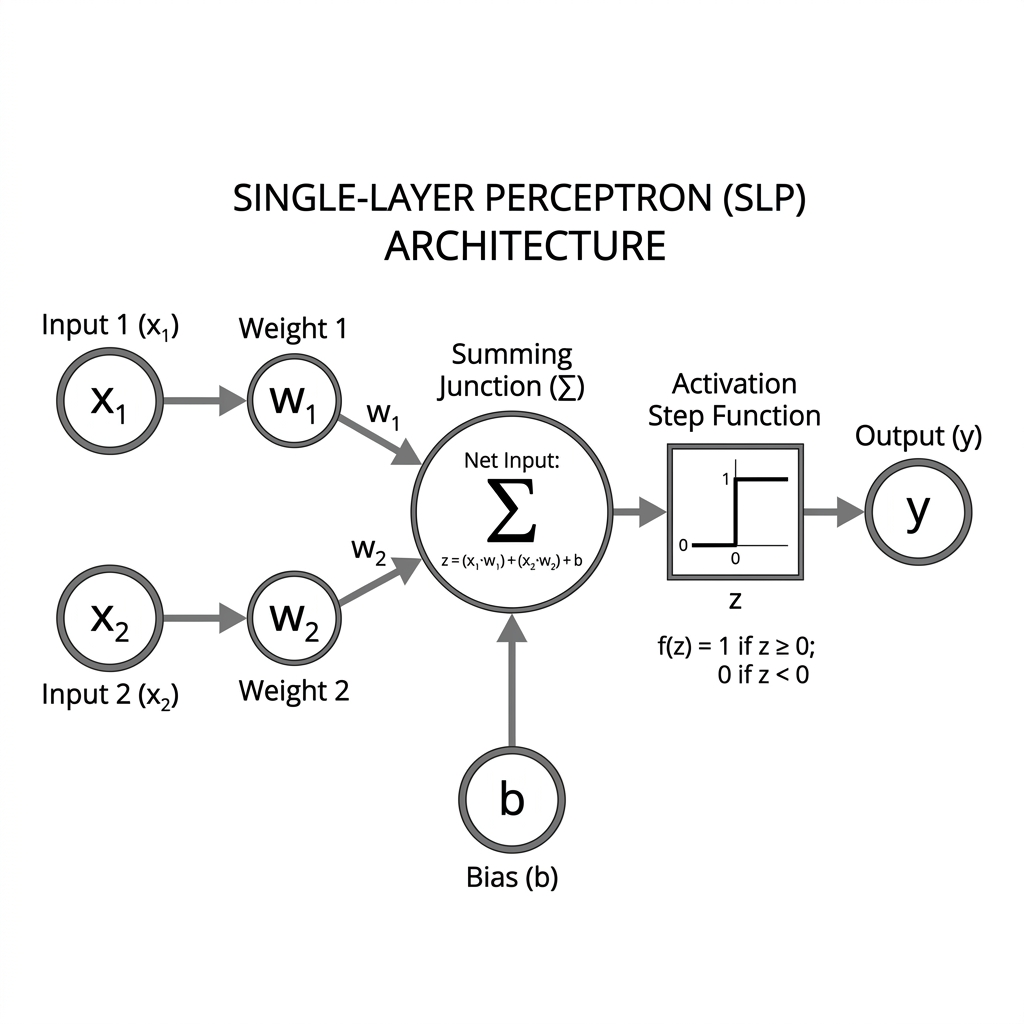
\includegraphics[width=0.7\textwidth]{arsitektur.png}
    \caption{Ilustrasi Arsitektur Perceptron}
    \label{fig:arsitektur}
\end{figure}

\subsection{Poin Analisis dari Kelompok Kami}
Berdasarkan data konvergensi di atas, kami merangkum beberapa poin analisis penting:
\begin{enumerate}
    \item \textbf{Pengaruh \textit{Learning Rate} pada Jumlah Epoch}: Dari hasil percobaan, kami mengamati bahwa penggunaan variasi \textit{learning rate} (0.1, 0.01, dan 0.001) ternyata tidak mengubah kecepatan konvergensi model. Baik pada angka berapapun, logika AND tetap konvergen pada epoch ke-6, dan logika OR konvergen pada epoch ke-4.
    \item \textbf{Skalabilitas dan Titik Inisialisasi}: Menurut analisis kami, hal tersebut terjadi karena inisialisasi awal bobot dan bias yang kami terapkan bermula dari titik 0 secara seragam. Akibatnya, seluruh perhitungan bobot hanya terkena efek perkalian proporsional dari $\alpha$. Karena syarat fungsi aktivasi kami bergantung pada nilai $net \ge 0$, maka hasil perkalian tersebut tidak akan pernah mengubah polaritas keputusan (positif atau negatifnya nilai $net$). Sebagai gambaran, $net = 0.2$ (saat $\alpha=0.1$) akan menghasilkan keputusan klasifikasi yang identik dengan $net = 0.002$ (saat $\alpha=0.001$).
    \item \textbf{Tingkat Kesulitan Keputusan}: Kami juga mencatat bahwa algoritma membutuhkan waktu pelatihan yang sedikit lebih lama untuk logika AND (6 iterasi penuh) dibandingkan logika OR (4 iterasi penuh). Hal ini mengindikasikan bahwa pencarian batas keputusan (\textit{decision boundary}) untuk memisahkan kelas-kelas pada kasus logika AND terbukti sedikit lebih rumit dari pada kasus logika OR.
\end{enumerate}

\newpage
\section{Perhitungan Manual (Contoh Skenario $\alpha = 0.1$)}

Untuk memperjelas bagaimana cara kerja pembaruan bobot dalam model kami, di sini kami menyajikan contoh simulasi perhitungan manual secara rinci langkah demi langkah. Kami mengambil contoh iterasi awal untuk skenario $\alpha = 0.1$.

\subsection{Perhitungan Manual untuk Logika OR ($\alpha = 0.1$)}
\textbf{Inisialisasi Awal}: $w_1 = 0, w_2 = 0, b = 0$

\subsubsection*{Langkah pada Epoch 1}
\begin{enumerate}
    \item Data Pertama ($x_1=0, x_2=0$, Target $=0$)
    \begin{itemize}
        \item $net = (0 \times 0) + (0 \times 0) + 0 = 0$
        \item Output model = $f(0) = 1$
        \item Error = $0 - 1 = -1$ (Karena terdapat error, kami melakukan \textbf{Update!})
        \item $w_1 = 0 + 0.1(-1)(0) = 0$
        \item $w_2 = 0 + 0.1(-1)(0) = 0$
        \item $b = 0 + 0.1(-1) = -0.1$
    \end{itemize}
    \item Data Kedua ($x_1=0, x_2=1$, Target $=1$)
    \begin{itemize}
        \item $net = (0 \times 0) + (0 \times 1) + (-0.1) = -0.1$
        \item Output model = $f(-0.1) = 0$
        \item Error = $1 - 0 = 1$ (Kembali terdapat error, kami melakukan \textbf{Update!})
        \item $w_1 = 0 + 0.1(1)(0) = 0$
        \item $w_2 = 0 + 0.1(1)(1) = 0.1$
        \item $b = -0.1 + 0.1(1) = 0$
    \end{itemize}
    \item Data Ketiga ($x_1=1, x_2=0$, Target $=1$)
    \begin{itemize}
        \item $net = (0 \times 1) + (0.1 \times 0) + 0 = 0$
        \item Output model = $f(0) = 1$
        \item Error = $1 - 1 = 0$ (\textit{Sudah tepat, tidak ada perubahan bobot})
    \end{itemize}
    \item Data Keempat ($x_1=1, x_2=1$, Target $=1$)
    \begin{itemize}
        \item $net = (0 \times 1) + (0.1 \times 1) + 0 = 0.1$
        \item Output model = $f(0.1) = 1$
        \item Error = $1 - 1 = 0$ (\textit{Sudah tepat, tidak ada perubahan bobot})
    \end{itemize}
\end{enumerate}

\textit{(Siklus pelatihan ini kami teruskan hingga akhirnya pada \textbf{Epoch ke-4}, model tidak menghasilkan error sama sekali di seluruh baris data. Saat itu tercapai, didapatkan bobot konvergen di titik $w_1=0.1, w_2=0.1, b=-0.1$)}.

\subsection{Perhitungan Manual untuk Logika AND ($\alpha = 0.1$)}
\textbf{Inisialisasi Awal}: $w_1 = 0, w_2 = 0, b = 0$

\subsubsection*{Langkah pada Epoch 1}
\begin{enumerate}
    \item Data Pertama ($x_1=0, x_2=0$, Target $=0$)
    \begin{itemize}
        \item $net = (0 \times 0) + (0 \times 0) + 0 = 0$
        \item Output model = $f(0) = 1$
        \item Error = $0 - 1 = -1$ (\textbf{Update!})
        \item $w_1 = 0, w_2 = 0, b = -0.1$
    \end{itemize}
    \item Data Kedua ($x_1=0, x_2=1$, Target $=0$)
    \begin{itemize}
        \item $net = (0 \times 0) + (0 \times 1) - 0.1 = -0.1$
        \item Output model = $f(-0.1) = 0$
        \item Error = $0 - 0 = 0$ (\textit{Tepat, tidak ada perubahan})
    \end{itemize}
    \item Data Ketiga ($x_1=1, x_2=0$, Target $=0$)
    \begin{itemize}
        \item $net = (0 \times 1) + (0 \times 0) - 0.1 = -0.1$
        \item Output model = $f(-0.1) = 0$
        \item Error = $0 - 0 = 0$ (\textit{Tepat, tidak ada perubahan})
    \end{itemize}
    \item Data Keempat ($x_1=1, x_2=1$, Target $=1$)
    \begin{itemize}
        \item $net = (0 \times 1) + (0 \times 1) - 0.1 = -0.1$
        \item Output model = $f(-0.1) = 0$
        \item Error = $1 - 0 = 1$ (\textbf{Update!})
        \item $w_1 = 0 + 0.1(1)(1) = 0.1$
        \item $w_2 = 0 + 0.1(1)(1) = 0.1$
        \item $b = -0.1 + 0.1(1) = 0$
    \end{itemize}
\end{enumerate}

\subsubsection*{Langkah pada Epoch 2}
\begin{enumerate}
    \item Data Pertama ($x_1=0, x_2=0$, Target $=0$)
    \begin{itemize}
        \item $net = (0.1 \times 0) + (0.1 \times 0) + 0 = 0$
        \item Output model = $f(0) = 1$
        \item Error = $0 - 1 = -1$ (\textbf{Update!})
        \item $w_1 = 0.1, w_2 = 0.1, b = -0.1$
    \end{itemize}
    \item Data Kedua ($x_1=0, x_2=1$, Target $=0$)
    \begin{itemize}
        \item $net = (0.1 \times 0) + (0.1 \times 1) - 0.1 = 0$
        \item Output model = $f(0) = 1$
        \item Error = $0 - 1 = -1$ (\textbf{Update!})
        \item $w_1 = 0.1, w_2 = 0, b = -0.2$
    \end{itemize}
    \item Data Ketiga ($x_1=1, x_2=0$, Target $=0$)
    \begin{itemize}
        \item $net = (0.1 \times 1) + (0 \times 0) - 0.2 = -0.1$
        \item Output model = $f(-0.1) = 0$
        \item Error = $0 - 0 = 0$ (\textit{Tepat, tidak ada perubahan})
    \end{itemize}
    \item Data Keempat ($x_1=1, x_2=1$, Target $=1$)
    \begin{itemize}
        \item $net = (0.1 \times 1) + (0 \times 1) - 0.2 = -0.1$
        \item Output model = $f(-0.1) = 0$
        \item Error = $1 - 0 = 1$ (\textbf{Update!})
        \item $w_1 = 0.2, w_2 = 0.1, b = -0.1$
    \end{itemize}
\end{enumerate}

\textit{(Siklus iterasi untuk model logika AND ini kami teruskan secara serupa, hingga puncaknya pada \textbf{Epoch ke-6} kami mencatatkan tidak ada lagi error (Error = 0) pada semua baris data. Hasil akhir yang dikonfirmasi adalah nilai konvergen di $w_1=0.2, w_2=0.1, b=-0.3$)}.

\end{document}
